\documentclass{article}

\usepackage[margin=2.5cm]{geometry}
\usepackage{amsmath,amssymb}
\usepackage{float}
\usepackage{graphicx}
\usepackage{fancyhdr}
\pagestyle{fancy}
\usepackage{tcolorbox,listings}
\usepackage{color}
\usepackage{hyperref}
\renewcommand\headrulewidth{1pt}
\usepackage{marvosym}
\usepackage{xcolor}
\usepackage{tikz}
\usepackage{babel}
\usepackage[french]{babel}
\usepackage[babel=true,kerning=true]{microtype}
\usepackage{afterpage}
\usepackage{wrapfig}
% \usepackage[colorlinks=true,urlcolor=blue]{hyperref}

\newcommand\myemptypage{
    \null
    \thispagestyle{empty}
    \addtocounter{page}{-1}
    \newpage
}

\usetikzlibrary{
    arrows,
    calc,
    shapes.geometric,
    shapes.misc,
    shapes.symbols,
    shapes.arrows,
    automata,
    through,
    positioning,
    scopes,
    decorations.shapes,
    decorations.text,
    decorations.pathmorphing,
    shadows}

\definecolor{darkWhite}{rgb}{0.94,0.94,0.94}

\lstset{
    backgroundcolor=\color{darkWhite},
    breakatwhitespace=false,
    breaklines=true,
    captionpos=b,
    commentstyle=\color{green},
    deletekeywords={...},
    escapeinside={\%*}{*)},
    extendedchars=true,
    keepspaces=true,
    keywordstyle=\color{blue},
    %language=Python,
    morekeywords={*,...},
    showspaces=false,
    showstringspaces=false,
    showtabs=false,
    stepnumber=1,
    stringstyle=\color{gray},
    tabsize=4,
}

\lstdefinestyle{frameStyle}{
    basicstyle=\sffamily,
    numbers=left,
    numbersep=20pt,
    numberstyle=\tiny\color{black}
}

\tcbuselibrary{listings,skins,breakable}

\newtcblisting{customFrame}{
    arc=0mm,
    top=0mm,
    bottom=0mm,
    left=3mm,
    right=0mm,
    width=\textwidth,
    listing only,
    listing options={style=frameStyle},
    breakable
}

\fancyhead[L]{ALLEMAND Fabien\\BALAKRISHNAN Sylvain\\BONNAIL Julie}
\fancyhead[C]{Mesurer les Infrastructures Routières}
\fancyhead[R]{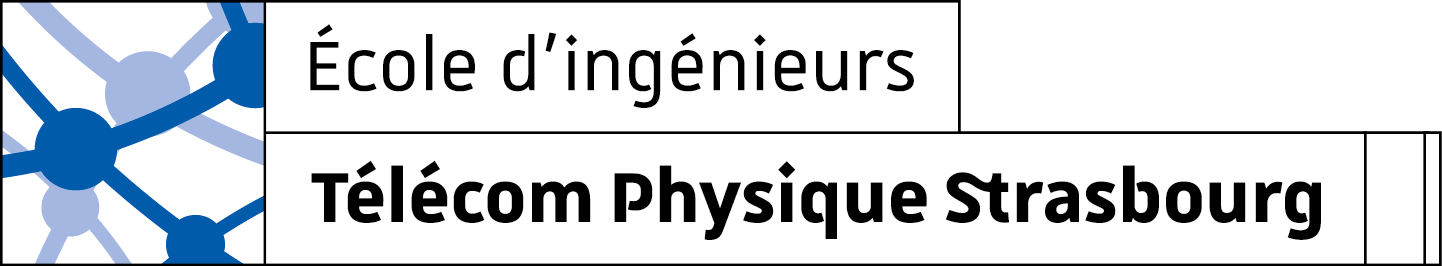
\includegraphics[scale=0.4]{../../common/logo_TPS_1.png}}
\fancyfoot[L]{Projet Ingénieur}
\fancyfoot[R]{\today}

\begin{document}

\thispagestyle{empty}
\addtocounter{page}{-1}
\begin{center}
    \baselineskip=50pt
    \vspace*{1cm}
    \textbf{{\Huge Projet Ingénieur}}\\
    \vspace*{0.25cm}
    \textbf{{\Huge Mesurer les Infrastructures Routières}}\\
    \vspace*{0.25cm}
    \begin{minipage}[c]{.46\linewidth}
        \centering
        \textbf{Equipe:}\\
        ALLEMAND Fabien\\BALAKRISHNAN Sylvain\\BONNAIL Julie
    \end{minipage}
\end{center}
\vspace*{0.1cm}

\begin{figure}[H]
    \centering
    \centerline{
\includegraphics[scale=.66]{../../common/logo_Alcatel_1.png}}
    \vspace*{0.1cm}
    \centerline{
\includegraphics[scale=1.25]{../../common/logo_TPS_2.png}}
\end{figure}

\newpage
\renewcommand{\contentsname}{Table des matières}
\tableofcontents

\newpage
\addcontentsline{toc}{section}{Liste des figures}
\renewcommand{\listfigurename}{Liste des figures}
\listoffigures

\newpage
\vspace*{0.01cm}

\section{Introduction}
Road infrastructures are key when it comes to traveling. Whether it is for daily commuting or one-time journeys, millions of people drive their vehicle on the road in order to go from a point A to a point B.\\
There is no denying that the state of deterioration of roads has a huge impact on the security of the drivers and passengers. An unexpected hole on a road can lead a conductor to change direction abruptly or loose control of the vehicle.\\
The effect of a poorly maintained road on vehicle is usualy overlooked but it seems logical that holes and bumps on a road are likely to cause damage on cars reducing security and increasing maintenance costs on the vehicle.\\
At a larger scale, transportations can be slown down by deteriorated roads meaning the entiere process of economical exchanges is running at a slower pace, hurting the economy of cities or even countries.\\
Finally, the military force of a country can be evaluated by the state of roads networks. In case of emergency, military forces need to move quickly. Once again, the state of the roads is a key factor.\\

The goal of this project is to develop an AI-based solution in order to facilitate road maintenance. By training an AI to recognize degradation on a road, road wrokers could more easily service roads and thus improve security and user experience.\\
In this study, the AI will be mostly trained on acceleration data measured on vehicles. In order to work properly, the model must be able to detect various degradations (bumps and obstacles, holes and cracks as well as gravel) independently of the type of vehicle the data is coming from.\\
For the purpose of the study, two methods will be used in order to collect acceleration data. First, using an Arduino and an IMU. In a second time, by using smartphones accelerometers.
% Different approaches can be used in order to collect acceleration data. The easiest is to create a simple device with an IMU that records data localy requiring human interaction in order to transfer data. Another way to access such type of data is to use accelerometers located in smartphones...
\\
As a proof of concept, a smartphone application will be created and will demonstrate the effectiveness of this road quality assessment method.\\

\section{Présentation du Projet}
L'état de dégradation des chaussées peut avoir un fort impact pour les usagers
et l'environnement. Ce projet a pour objectif de développer une solution
informatique pour améliorer les conditions de conduites face aux routes mal
entretenues.

\subsection{Enjeux}
En 2017, près de 75\% des actifs français utlisent une voiture pour effectuer
leurs
déplacements quotidiens notamment pour se rendre sur leur lieu de travail
\cite{insee}. Ce sont donc 18,1 millions d'usagers qui parcourent le réseau
routier français régulièrement. Selon des études plus récentes, la proportion
de travailleurs utilisant leur voiture pour effectuer les trajets
domicile-travail a augmenté sous l'effet de la crise sanitaire liée à la
Covid-19 \cite{covid}, les français ne se sentant plus en sécurité dans les
transports en commun.
De nos jours, les véhicules routiers représentent plus de 80\% des
déplacements des français lors des vacances \cite{vacances}.
Selon l'Insee, il y a 37,9 millions de véhicules actuellement en service en
France.
Assurer la sécurité et le confort de l'ensemble des usagers lors de leurs
déplacements personnels ou professionnels est donc une priorité. Or 30\% des
accidents de la route mortels sont causés par des déformations sur la chaussée
\cite{europe1}. Ce chiffre pourrait augmenter avec l'arrivée des véhicules
autonomes sur les routes. Ces derniers pourraient être déstabilisés par
certains défauts sur les routes.
Néanmoins, selon le dernier rapport de l'ONR le budget consacré à l'entretien
des routes ne cesse de diminuer \cite{onr} alors que la qualité du réseau
routier se dégrade \cite{tf1}.\\

Outre le confort et la sécurité, les défauts sur les chaussées impactent aussi
les frais d'entretiens des véhicules. Selon une étude menée aux Etats Unis
d'Amérique, les réparations engendrées par le mauvais état des routes
représentent plusieurs centaines d'euros par voiture par an.\\

D'autres études dénoncent aussi un coût environnemental. Les dégâts et les
réparations sur les véhicules ne sont pas sans impact sur la nature
\cite{pneus} et les conditions des routes peuvent drastiquement modifier le
comportement du véhicule ce qui peut induire une plus forte emission de gaz à
effet de serre.\\

Finalement, l'état et la qualité du réseau routier ont une influence sur la
compétitivité économique et militaire d'un pays : un pays ayant un réseau
routier médiocre ne pourra pas faire transiter des marchandises suffisamment
rapidement et sera donc moins compétitif \cite{economique}.

% -Sécurité (Dégradation rapide)
% -Confort (Dégradation rapide)
% -Cout
% -Pollution
% -Compétitivité

\subsection{Mise en \oe{}uvre}
Etant donné l'étendue des réseaux routiers et leur rapide évolution, mobiliser
une équipe de personnel d'entretien afin de parcourir l'ensemble des routes, de
façon régulière, ayant pour mission de repérer et réparer les dégradations
n'est pas une
solution viable en terme de coût financier et environnemental. De plus, cette
méthode ne fournirait pas nécessairement de bons résultats puisque certaines
dégradations pourraient ne pas être vues ou tout simplement négligées par les
ouvriers.\\

Le but est donc de créer un système informatique capable d'analyser en continu
l'état de la
route et de transmettre en temps réel les éventuels dégâts repérés.\\

La collecte de donnée sous forme participative s'annonce comme l'unique
alternative aux équipes de techniciens balayant le réseau routier car les
images satellites
n'offrent pas suffisamment de précision pour repérer des dégradation à
l'échelle d'une route et il n'est pas envisageable de placer des capteurs pour
surveiller l'état de l'ensemble d'un réseau routier. Collecter dans une base de
donnée communautaire des informations sur les routes permet de recouvrir
le réseau selon les dimensions spaciales et temporelle.\\

Afin de limiter le coup de déploiement du système, la collecte de donnée
peut être réalisée à l'aide d'un smartphone. Les téléphones portables
actuels contiennent de nombreux capteurs et une puissance de calcul non
négligeable. La collecte de données se fait au travers d'une
application développée à cet effet. Le choix du smartphone plutôt qu'un
appareil spécialisé permet aussi de limiter l'impact environnemental du
projet.\\
Cette même application sera utilisée par les ouvriers voiries pour prendre
connaissance de l'état courant de la route (Figure \ref{syst_1}).\\

\begin{figure}[H]
    \centering
    \begin{tikzpicture}[>=stealth,yscale=2,xscale=1.4]
        % Nodes
        \node(conducteur) at (0,0)[rectangle,draw,text centered,align=center]
        {Conducteur};
        \node(app) at (5,0)[rectangle,draw,text centered,align=center]
        {Application};
        \node(entretien) at (10,0)[rectangle,draw,text centered,align=center]
        {Ouvrier voiries};
        % Links
        \draw[-] (conducteur) -- (app);
        \draw[-] (app) -- (entretien)
    \end{tikzpicture}
    \caption{Description du fonctionnement du système}
    \label{syst_1}
\end{figure}

Un traitement par image est envisageable. Une caméra embarquée a
l'avantage de balayer une grande surface d'un réseau rapidement et de façon
régulière. Cependant, la qualité de l'image lors du déplacement du véhicule
dans des conditions d'éclairage variables n'est probablement pas suffisante
pour détecter les dégradations les plus fines. De plus l'utilisation d'une
caméra entraine des contraintes supplémentaires pour l'utilisateur:
positionnement de la caméra, espace de
stockage, consomation énergétique...\\

En revanche la collecte de données accélérométriques peut être réalisée à
moindre coup. Il est possible d'utiliser l'accéléromètre contenu dans un
smartphone sans imposer trop de
contraintes à un utilisateur. Par ailleurs, l'espace mémoire pour enregistrer
les données est significativement plus faible. Les données recueillies
contenant notamment l'accélération verticale permettront de repérer des défauts
sur la chaussée. Il est important de remarquer que seules les dégradations sur
lesquelles l'utilisateur roulera seront détectées.\\

Le traitement des données collectées pourrait se faire localement grâce à la
puissance de calcul des processeurs portables. Cependant, envoyer les données à
un serveur qui prend en charge l'analyse libère le smartphone de l'utilisateur
de cette tâche.\\

Afin d'améliorer les conditions de conduites, toute dégradation de la chaussée
doit être signalée au plus vite au personnel chargé de l'entretien. Suite à
l'analyse, le
personnel peut être prévenu grâce à une notification provenant de l'application
pour smartphone comme décrit sur la Figure \ref{syst_2}.\\

% La détection de défauts sur les infrastructures routières peut être réalisée
% grâce à une analyse de données recueillies sur les chaussées. Sachant que
% l'état d'une chaussée peut se dégrader rapidement, ces données doivent être
% recueillies régulièrement. On peut donc envisager que la collecte de données
% soit réalisée de façon participative au travers de conducteurs volontaires en
% utilisant une application pour smartphone.\\

\begin{figure}[H]
    \centering
    \begin{tikzpicture}[>=stealth,yscale=2,xscale=1.4]
        % Nodes
        \node(conducteur) at (0,0)[rectangle,draw,text centered,align=center]
        {Conducteur};
        \node(app) at (5,0)[rectangle,draw,text centered,align=center]
        {Application};
        \node(entretien) at (10,0)[rectangle,draw,text centered,align=center]
        {Ouvrier voiries};
        \node(serveur) at (5,1)[rectangle,draw,text centered,align=center]
        {Serveur};
        % Links
        \draw[->] (conducteur) -- (app) node[midway,above]{Données à analyser};
        \draw[->] (app) -- (entretien) node[midway,above]{Notification};
        \draw[-] (app) -- (serveur);
    \end{tikzpicture}
    \caption{Description du fonctionnement du système (Analyse)}
    \label{syst_2}
\end{figure}

Le traitement des données sur le serveur repose sur un système d'intelligence
artificelle permettant de classer les signaux accélérométriques reçus. Etant
donné que le modèle est uniquement sur le serveur, il peut facilement être
amélioré avec de nouvelles données d'entrainement. Pour cela, un ouvrier peut
confirmer une dégradation signalée par l'application (Figure \ref{syst_3}). Cela permet d'obtenir de
nouvelles données labellées.\\

\begin{figure}[H]
    \centering
    \begin{tikzpicture}[>=stealth,yscale=2,xscale=1.4]
        % Nodes
        \node(conducteur) at (0,0)[rectangle,draw,text centered,align=center]
        {Conducteur};
        \node(app) at (5,0)[rectangle,draw,text centered,align=center]
        {Application};
        \node(entretien) at (10,0)[rectangle,draw,text centered,align=center]
        {Ouvrier voiries};
        \node(serveur) at (5,1)[rectangle,draw,text centered,align=center]
        {Serveur};
        % Links
        \draw[<-] (conducteur) -- (app) node[midway,above]{Notification};
        \draw[<-] (app) -- (entretien) node[midway,above]{Données à conserver};
        \draw[-] (app) -- (serveur);
    \end{tikzpicture}
    \caption{Description du fonctionnement du système (Collecte)}
    \label{syst_3}
\end{figure}

\section{State of the Art}
Artificial intelligence is being used more and more and is becoming more and more powerful. Current AI models are capable of responding to complex tasks with solid repercussions. The applications are diverse: audio signal processing, medical image classification, or defect detection on production lines.\\
There are already many applications regarding roads notably: drunk driving detection \cite{drunk_2}\cite{drunk_1} or vehicles control and monitoring \cite{xxii} without forgetting autonomous vehicles which do not cease evolving \cite{vehicle_1}.\\
Road condition analysis and damage detection have been the subject of much research. Some researchers use external accelerometers in a series of filters to identify potholes or railway crossings via time-domain analysis only \cite{road_4}\cite{road_5}. Data are generally used in the frequency domain \cite{road_2}\cite{road_1}.\\
The use of smartphone accelerometric sensors has already proven to be a relevant alternative to external sensors \cite{road_3}. Systems that performs rich sensing using smartphones used by people on regular day-to-day driving, where several sensing modalities, such as accelerometers, microphones, GSM radio and GPS are used to monitor both road and traffic conditions \cite{road_6}.\\
Other machine learning applications use accelerometric data. The rise of connected watches has revealed the usefulness of this data type for fall detection \cite{fall_1} \cite{fall_2} using edge artificial intelligence architecture \cite{fall_3}.\\

% The analysis of road quality measured by longitudinal has been studied for road and aeronautical pavements \cite{road_7}.



\section{Objectifs}
Pour mener à bien notre projet, il est envisagé d'entraîner un premier modèle avec des données
d'entraînement. Ces données seront recueillies à l'aide d'outils qui sont à disposition (Arduino, robot téléguidé).
Ce modèle devra permettre d'analyser de nouvelles données accélérométriques et de les classer par type de dégradation.
Pour optimiser le modèle et éviter au maximum les fausses alertes, il faut que le modèle puisse s'améliorer
au cours du temps à l'aide de nouvelles données enregistrées. Pour cela, l'intelligence artificielle mise en \oe{}uvre devra être compatible avec l'\textit{online learning} (apprentissage
incrémental grâce à des nouvelles données).
De plus pour que chaque acteur puisse contribuer de la meilleure des manières, il est envisagé de réaliser une application mobile d'utilisation simple et disponible à la plupart des conducteurs.

\section{Périmètre du Projet}

\section{Risques}
Il existe de nombreux risques pouvant impacter le développement et par la suite le bon fonctionnement du système basé sur l'application. Le but de cette section et d'appréhender ces risques et de proposer des solutions afin de les éviter ou de les corriger si besoin.\\

Dans un premier temps, de nombreux facteurs peuvent impacter la qualité des données recueillies.\\
Il faut que le système soit capable de détecter si les données correspondent bien à un enregistrement effectué dans un véhicule. De même l'utilisaton du smartphone par un passager fausserait les données. Les données collectées par l'utilisateur par inadvertence doivent être ignorées par un système de détection d'outliers.\\
La position du téléphone lors de l'enregistrement doit être prise en compte. L'application doit être capable de connaitre l'orientation du téléphone pour en extraire les données d'accélération verticale. (Cela évite une contrainte supplémentaire pour l'utilisateur qui devrait dans le cas contraire fixer son téléphone dans une position précise et prédéfinie).\\
La position du smartphone dans le véhicule risque d'impacter les données accélérométriques : moins de fortes secousses à proximité des essieux. L'intelligence artificielle pourrait être entrainée sur des données récoltées à différentes position dans le véhicule afin de contrer ce biais.\\
Finalement, un instrulment mal calibré peut fournir des données erronées. Il faut donc effectuer régulièrement des phases de calibration de l'appareil.\\

L'intelligence artificielle entrainée ne sera sûrment pas infaillible mais il faudra faire en sorte de limiter les cas de faux positifs (objets égarés sur la routes ou dégradation temporaries dues à des travaux) et les faux négatifs (obstacles marginaux, dégradation en bord de route ou en dehors du passage des roues).\\

Finalement, le système peut souffrir d'une mauvaise adaptabilité. Nous souhaitons dans un premier temps travailler avec un robot téléguidé dont la strucure est différente d'un vrai véhicule. De plus chaque véhicule possède une géométrie et un système d'amortisseurs différents donc la réaction de chaque véhicule face aux dégradations est unique.\\


\section{Ressources et Rôles}

\section{Planning Initial}

\section{Conclusion}
Having understood the subject, its issues and constraints, having created supports to use the sensors and having started to collect our first accelerometric data, we can move on to the next stage of the project. Between now and the next review, we plan to analyze the data collected. This will give us an idea of the artificial intelligence model to use. Once this is done, we will have to collect more data so that the selected models are trainable and as accurate as possible. We will then be able to compare the models and choose which one(s) we will select for the rest of the project. Finally, we will also start to develop the mobile application because it can be done in parallel with the artificial intelligence part.

\newpage
\vspace*{0.01cm}
\addcontentsline{toc}{section}{Bibliographie}
\renewcommand{\refname}{Bibliographie}
\bibliographystyle{plain}
\bibliography{bibliography.bib}

\end{document}